\documentclass[a4paper,UKenglish,cleveref, autoref, thm-restate]{lipics-v2021}
\hideLIPIcs

\newcommand{\ident}[1]{\textsf{#1}}
\newcommand{\ddident}[1]{\guillemotleft\ident{#1}\guillemotright}
\newcommand{\sigmaN}{\sigma_0}
\newcommand{\select}{\textnormal{\ident{choose}}}
\newcommand{\choices}{\textnormal{\ident{choices}}}
\newcommand{\op}{\textit{op}}
\newcommand{\vect}[1]{\lbrack #1 \rbrack}
%\newcommand{\preview}{\textnormal{\ident{preview}}}
%\newcommand{\links}{\textnormal{\ident{links}}}
\DeclareMathOperator{\argmax}{arg\,max}

\bibliographystyle{plainurl}
\title{The Choose-Your-Own-Adventure Calculus (Pearl/Brave New Idea)}

\author{Tomas Petricek}{Charles University, Prague, Czechia}{tomas@tomasp.net}{0000-0002-7242-2208}{}
\author{Jan Liam Verter}{Charles University, Prague, Czechia}{todo@todo}{}{}
\author{Mikoláš Fromm}{Charles University, Prague, Czechia}{todo@todo}{}{}
\ccsdesc[500]{Software and its engineering~General programming languages}
\keywords{Interactive programming systems, Type providers, Proof assistants}
\nolinenumbers

% \funding{funding}
% \acknowledgements{I want to thank \dots}
\authorrunning{Authors}

\begin{document}

\maketitle

\begin{abstract}

Some of the most remarkable results in mathematics reveal connections between different
branches of the discipline. The aim of this paper is to point out a modest, but still
remarkable, similarity between a range of different interactive programming systems.

~

use a simple formal mathematical model
that we call \emph{the choose-your-own-adventure calculus} to


todo

% and enable a transfer of ideas between them

\end{abstract}

\newpage

\section{Introduction}

Multiple interactive programming systems, ranging from code editors for object-oriented programming
languages to data exploration systems and interactive proof assistants, exhibit a remarkably
similar pattern of interaction. They offer the user, who can be a programmer, a data scientist
or a proof writer, a range of choices that the user can select from in order to complete their
program, script or proof. The user can initiate the interaction iteratively, using it to
create and refine a larger part of their program.

There are subtle differences between different implementations of the general pattern. In some
systems, the resulting source code will contain a trace of the choices made by the user.
For example, when choosing an item from a list of class members, the code will contain the member
name. In some systems, the interaction results in a block of code that can be included in the
source file, but does not include a trace of the interaction. For example, invoking a proof search
or case split in Idris \cite{brady-2015-idris} constructs a well-typed program, but leaves no trace
of the command used to construct it.
%
The nature of the generated options also varies. The list of choices may include all possible
options that are valid at a given location, or it may list only a subset of the valid options.
In some cases, it may also include incorrect options as, for example, in auto-completion
for dynamic languages \cite{frolich-2024-autocomplete}.

The aim of this paper is paper is to formally capture the recurring interaction pattern:

\begin{enumerate}
\setlength{\itemsep}{5pt}
\item We motivate the formalism by reviewing four different systems that implement a variation on the
interaction pattern. These include type providers for data access in F\# \cite{syme-2013-inforich},
type providers for data exploration in The Gamma \cite{petricek-2022-thegamma,petricek-2017-dotdriven},
AI assistants for semi-automated data wrangling \cite{petricek-2023-aias} and tooling for
interactive proof assistants \cite{altenkirch-1994-alf,brady-2015-idris,verter-2024-mixed} (Section~\ref{sec:motivation}).

\item We introduce the \emph{choose-your-own-adventure calculus}, which is a small formal structure
that models an interactive system where a user constructs a program by repeatedly choosing from a list
of options offered by the system (Section~\ref{sec:calculus}).

\item The calculus allows us to make the aforementioned subtle differences precise. We define the
notions of \emph{correctness} and \emph{completeness} for the choose-your-own-adventure calculus.
To distinguish the different ways of embedding the interactions in the edited programs, we
also formally define \emph{internal} and \emph{external} mode of system integration.

\item We show that various programmer assistance tools, such as search and AI-based recommendations
can be built on top of the primitives offered by the calculus, showing how the
choose-your-own-adventure calculus supports of transfer of ideas across different kinds of
interactive programming systems.
\end{enumerate}

The main contribution of this paper is conceptual rather than technical. We capture a
pattern that is perhaps not surprising in retrospect, but that is easy to overlook until it is
given a name. We use formal programming language theory methods to precisely describe
interesting aspects of the pattern. Moreover, our work also confirms that programming
language theory methods can be extremely effective for studying not just \emph{programming
languages}, but also interactive \emph{programming systems}~\cite{jakubovic-2023-techdims}.

\newpage

\begin{figure}[t]
  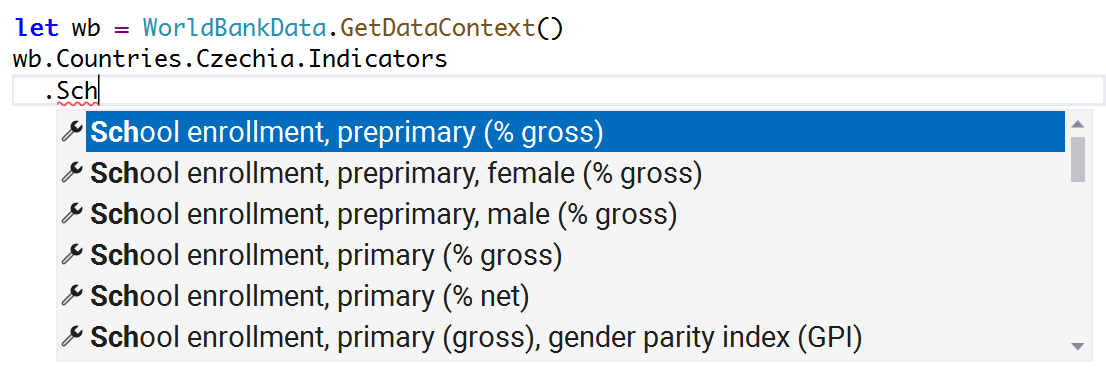
\includegraphics[width=0.7\textwidth]{fig/worldbank.png}
  \caption{F\# code editor showing completions offered by the World Bank type provider.}
  \label{fig:worldbank}
\end{figure}

\section{Motivation}
\label{sec:motivation}

Computer scientists studying programming have long focused on programming languages as syntactic
entities, sometimes neglecting the interactive environments in which they are inevitably
embedded \cite{rpg-2012-revolution}. Notably, in many of the motivating examples that we draw
from in this section, the interactive aspect of the system is only described in supplementary
materials \cite{brady-2015-idris,syme-2013-inforich,altenkirch-1994-alf}. Only recently, programming
language theory started to be used to study interactive environments
\cite{adams-2025-grove,mayer-2018-bidirectional}. Our work contributes to this research direction.

The following sections review four different instances of the choose-your-own-adventure
interaction pattern. In all of those, an interactive editor offers the user some kind of~a~com\-pletion list during working with the system.

\subparagraph{Type providers.}

F\# type providers \cite{syme-2013-inforich} are a mechanism for integrating external data
sources into the F\# type system. A type provider is a compiler extension, loaded and
executed at compile-time and at edit-time. It can run arbitrary code to read the structure of
external data and use it to generate a suitable statically-typed representation of the
data, typically as objects with members. Type providers can, for example, infer the type from a
sample JSON \cite{petricek-2016-fsdata} or read a database schema.

The example in Figure~\ref{fig:worldbank} shows a simple type provider for accessing information
from the World Development Indicators database. The provided \ident{wb} object allows the programmer
to access any indicator of any country in the database by choosing an appropriate \ident{[Country]}
and an \ident{[Indicator]} in a chain of members
\ident{wb}.\ident{Countries}.\ident{[Country]}.\ident{Indicator}.\ident{[Indicator]}.
The result is a time series with values for the given indicator and a country. More generally,
the example can be seen as a special case of a type provider for slicing n-dimensional
data cube \cite{petricek-2022-thegamma} -- we choose a fixed value for two of the three
dimensions (country, indicator, time).

When using the type provider, the user types the first line of code and triggers auto-completion
by typing \ident{wb} followed by the dot. The rest of the code is constructed by choosing an
option from a list and typing another dot.\footnote{This interaction pattern has been
lightheartedly called \emph{dot-driven development} by Phil Trelford \cite{seemann-2021-head}.}


\newpage

\begin{figure}[t]
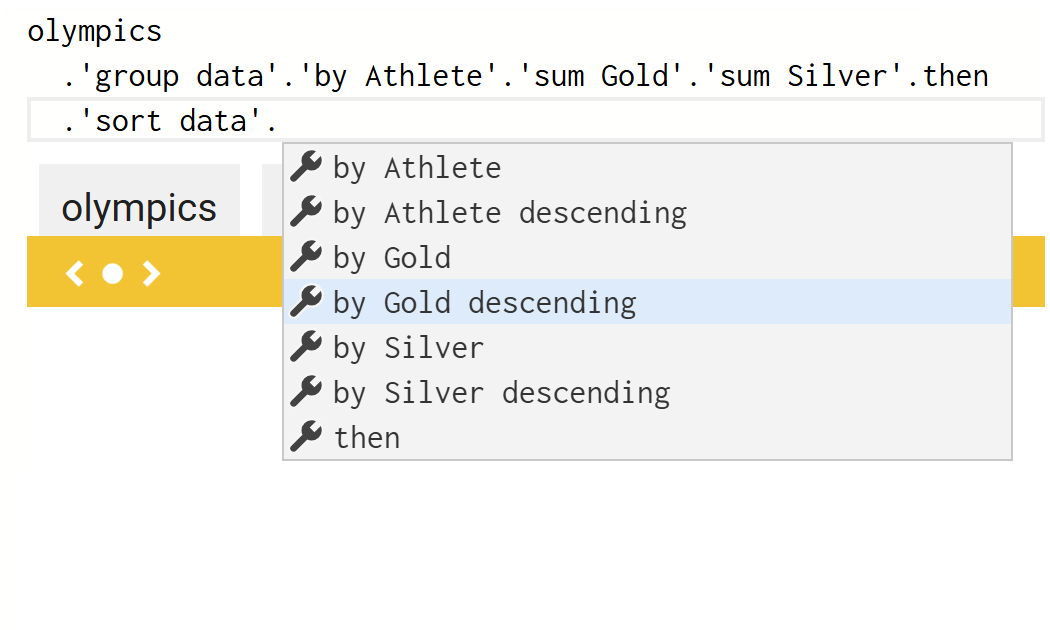
\includegraphics[width=0.48\textwidth]{fig/thegamma1.png}~~
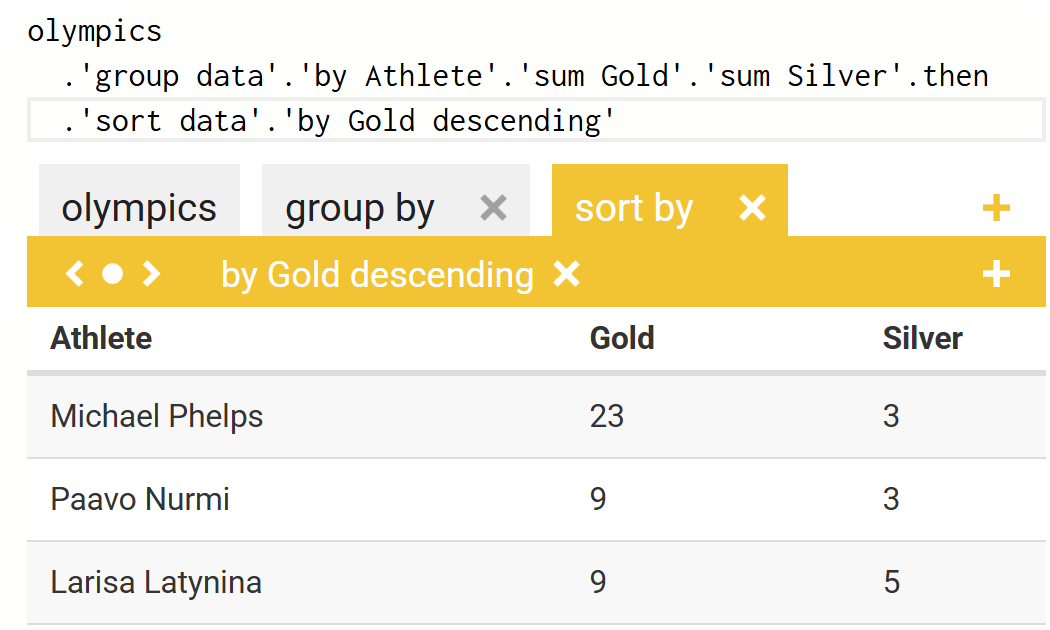
\includegraphics[width=0.48\textwidth]{fig/thegamma2.png}
\caption{Constructing a query in The Gamma. We count the number of gold and silver medals for
each athlete and sort the data by the number of gold medals.}
\label{fig:thegamma}
\end{figure}

\subparagraph{Data exploration.}

The Gamma~\cite{petricek-2022-thegamma} is a programmatic data exploration environment
for non-programmers. In The Gamma, type providers are the primary programming mechanism. They
are used not just for data access, but also for constructing queries.

The type provider shown in Figure~\ref{fig:thegamma} lets the user construct an SQL-like query by
repeatedly choosing operations and their parameters \cite{petricek-2017-dotdriven}. It keeps track
of the schema and uses it to generate all possible valid parameters. When sortin data, it generates
an object with two members for each columns -- one for ascending and one for descending sort.
Similarly, the grouping operation first offers all columns as possible grouping keys and then
lets the user choose from a range of pre-defined aggregations (sum, count, average, concatenate).
The system also evaluates the query on the fly, providing a live preview during editing \cite{petricek-2020-live}.

The interaction pattern is the same as before. After the usertriggers auto-completion, they
repeatedly select an operation and its parameters to construct a query. One notable difference
is that the structure of the generated types is potentially infinite (the user can keep adding
further operations) and so the types are generated lazily.

\subparagraph{AI assistants.}

The third instance of the choose-your-own-adventure interaction pattern comes from the work on
semi-automatic data wrangling tools known as AI assistants \cite{petricek-2023-aias}.
An AI assistant guides the analyst through a data wrangling problem such as reconciling mismatched
datasets, filling missing values or inferring data format and types. An AI assistant solves
the problem automatically and suggests an initial data transformation, but it also generates a
number of constraints that the user can choose from to refine the initial solution. If the initial
solution is not correct, the user chooses a constraint and the AI assistant runs again, suggesting
a new data transformation that respects the constraint.

Figure~\ref{fig:aia} shows an example. It uses the datadiff \cite{sutton-2018-datadiff} AI
assistant, running in a Wrattler notebook \cite{petricek-2018-wrattler}, to merge broadband
quality data published by Ofcom for two subsequent years. The format of the CSV files for the
two years differs. Columns were added, removed, renamed and their order has changed. In the
example, we selected 6 columns from the year 2015 and want to find matching data from 2014.

When the AI assistants runs automatically, it correctly maps the numerical columns, but it
incorrectly maps the \ident{Urban.rural} (2014) column to \ident{Nation} (2015). This happens
because both columns are categorical and have three values with similar distribution. A data
analyst can easily spot the mistake. They click the ``+'' button to add a constraint and choose
\ident{Don't match Urban.rural and Nation} to specify that the two columns should not be matched.
Datadiff then runs again and finds the correct matching.

\begin{figure}[t]
  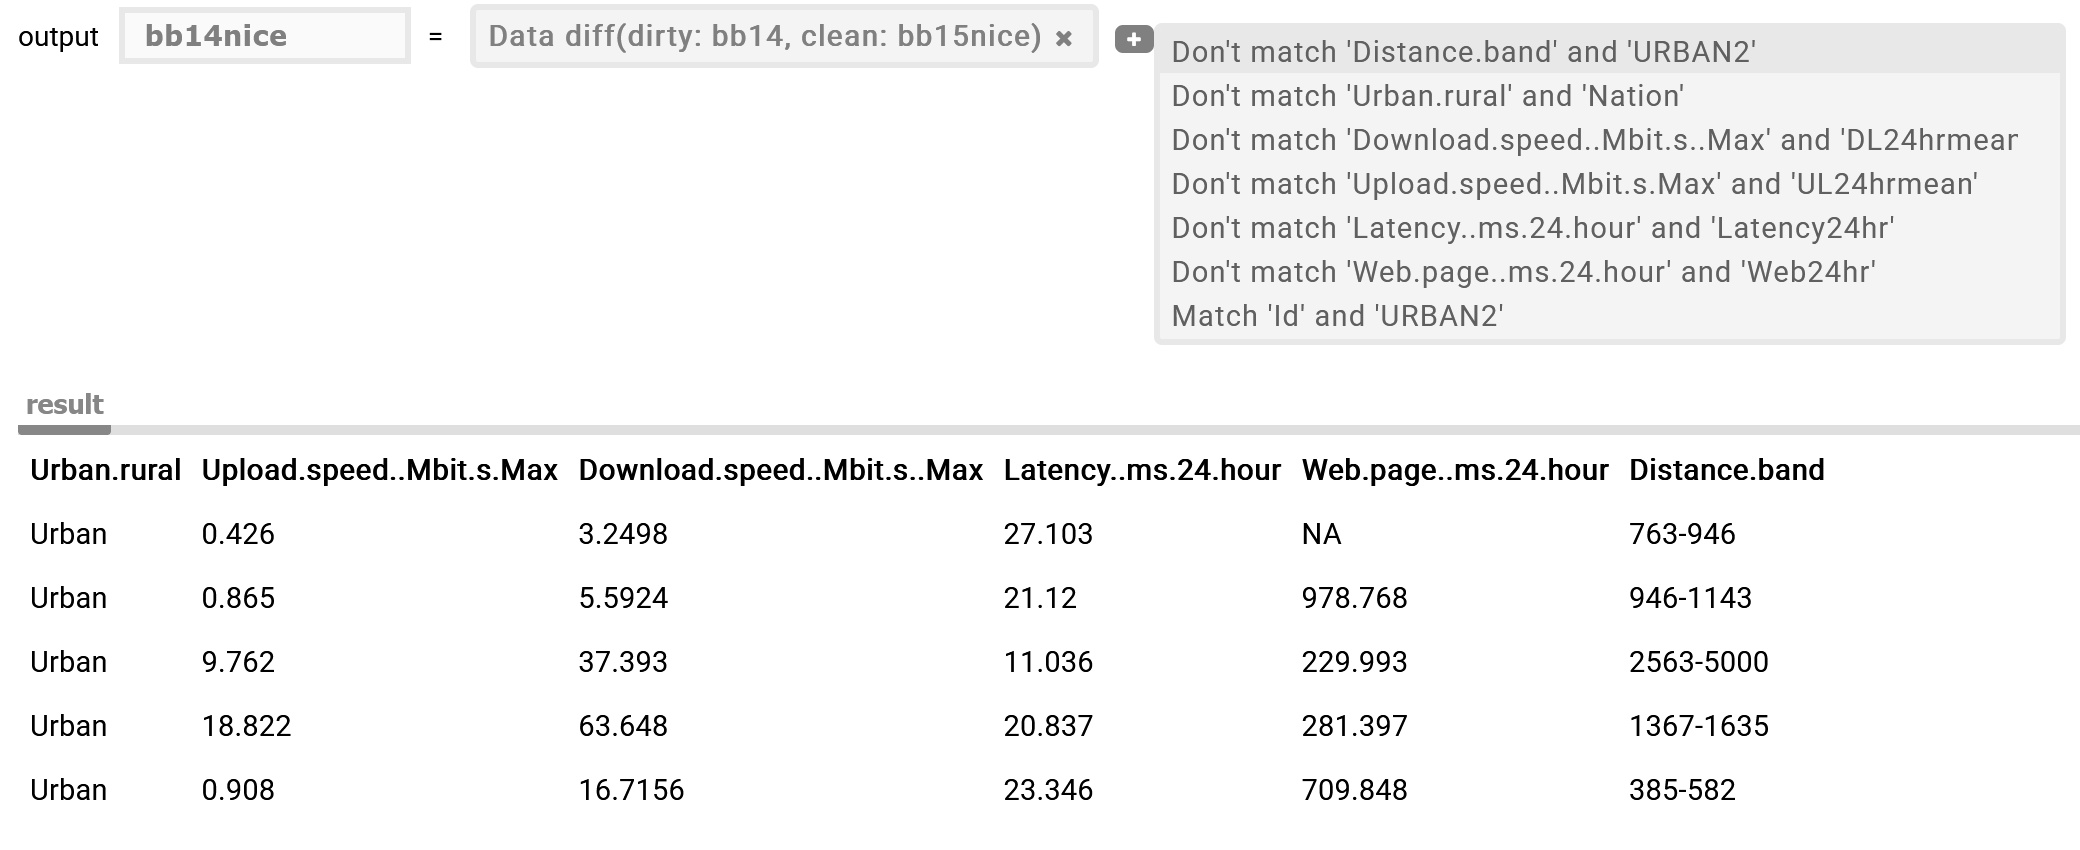
\includegraphics[width=0.9\textwidth]{fig/aia.png}
  \caption{Using the datadiff AI assistant to reconcile the structure of the two datasets.
    The user is offered a list of constraints to prevent or force matching between specific columns.}
  \label{fig:aia}
\end{figure}

~

The interaction patter is the same as in the previous two cases. The analyst constructs the
correct data transformation by repeatedly choosing from a list of options, until they obtain
the desired result. However, the way the interaction pattern is implemented differs.
First, in the case of type providers, we are gradually constructing a program by adding operations to
a method chain. Now, the AI assistant synthesizes a data transformation (program) and we are
gradually adding constraints to control the synthesis. Second, in the case of type providers,
the completion list offered all possible members of the object. Now, the list offers
constraints recommended by the AI assistant which may not be complete.

\newpage

\begin{figure}[t]
  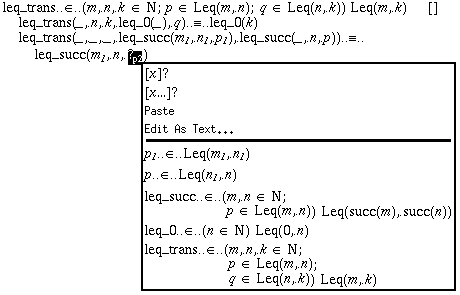
\includegraphics[width=0.6\textwidth]{fig/alf.png}
  \caption{Constructing a proof of the transitivity of the $\leq$ relation in the \textsc{Alf}
    editor. The user is offered a range of variables and constructors in scope at the current
    location. \cite{altenkirch-1994-alf}}
  \label{fig:alf}
\end{figure}


\subparagraph{Interactive theorem provers.}
A fourth example of the choose-your-own-adventure interactive pattern can be found in interactive
theorem provers. When writing programs in systems like Idris \cite{brady-2021-idris2}, the
user typically works by stating the desired conclusion and filling the implementation with a hole.
The system provides a range of interactive editing capabilities to fill the holes \cite{mcbride-1999-dependently}.
It can, for example, generate a case split or search for a proof \cite{brady-2015-idris}.

Systems like Idris provide key bindings to invoke the completions, but the functionality could
also be offered through a user interface. An example that illustrates this is the interactive editor
for the \textsc{Alf} theorem prover \cite{magnusson-1994-alf}, which is based on the refinement of
an incomplete proof object \cite{altenkirch-1994-alf}. This is illustrated in Figure~\ref{fig:alf}.
The user is proving the transitivity of the $\leq$ relation for Peano arithmetic natural numbers.
They pattern match on the proof argument $p$ and complete the first branch. For the second branch,
they need to fill a hole $?_{p2}$ (called a wildcard in \textsc{Alf}). They trigger a completion
and a pop-up menu shows the available variables and constructors, including \ident{leq\_trans} that
can be used to complete the proof. After choosing \ident{leq\_trans}, two new holes are generated
for its arguments. Those can be, again, filled interactively, by choosing $p_1$ and $p$ from the
completion.

The interaction pattern is again the same. The user repeatedly triggers a completion and uses
it to refine and complete their proof by filling holes. There are subtle differences too. Unlike
with AI assistants, each completion directly refines the proof that the user is editing. Unlike
with type providers, a completion may generate multiple new holes, rather than just adding to a
chain of operations.

The \textsc{Alf} editor is a historical example, but a similar user interface could be built for
systems like Idris or Coq. The two would work differently. As in \textsc{Alf}, Idris source code
represents the proof itself and a completion would replace a hole with a suggested term. In Coq,
the proof is a series of tactic invocations and so selected completions would be added to this
list and would form a trace of the interaction with the user.

\newpage

\section{Formal model}
\label{sec:calculus}

A system that implements the choose-your-own-adventure interaction pattern repeatedly offers
the user a range of options to choose from. Each of the options is designated by an identifier.
The system also maintains a state during the process which determines subsequent options. The state
may not be visible to the user, but the user can always explicitly request the program constructed
so far.

We can think of the interaction with the system as navigating through a tree structure, starting
from a root and choosing one of the possible branches in each step.\footnote{Serving as another
evidence for the surprising effectiveness of the concept of a tree \cite{nesetril-2005-strom}.}
In the following definition, the key $\choices$ operation can thus be seen as returning
branches of a given node.

\begin{definition}[Choose-your-own-adventure system]\label{def:calculus}
Given expressions $e\in \mathbb{E}$ and states $\sigma \in \Sigma$, a choose-your-own-adventure
system is a pair of operations \choices, \select\ such that:

\vspace{-0.25em}
\raggedright
\begin{itemize}
  \item $\choices(\sigma) = \{\iota_1\mapsto\sigma_1, \ldots, \iota_n\mapsto\sigma_n\}$ is
    an operation that takes a state and \\ generates options designated by an identifier $\iota_i$
    and represented by a state $\sigma_i$,
  \item $\select(\sigma) = e$ is an operation that returns generated program for a given state.
\end{itemize}
\end{definition}

The definition is not a programming language calculus in the usual sense in that it does not
define a concrete syntax with reduction rules. It is an abstract algebraic structure that captures
the structure of a system that supports the choose-your-own-adventure interaction pattern.
The definition is close to that of an AI assistant \cite{petricek-2023-aias}, which is written
using a language specific for the data wrangling domain (such as cleaning scripts or input and
output data) but is structurally similar. It is also worth noting that the definition may describe
not just trees, but also graphs with cycles -- a system can return to an already visited state.
This is not practically useful, but it does not pose a theoretical problem.

\subparagraph{External mode of embedding.}
One of the subtle questions about the choose-your-own-adventure pattern raised in the introduction
concerns the different ways in which a trace of the interaction is embedded in the interactively
constructed program. In the \emph{external mode}, the interaction results in code that becomes a
part of the edited program, but it is not possible to reconstruct the steps used to generate the code.

The choose-your-own-adventure interaction pattern is typically used to complete a partial program.
To model this, we assume that the host language has a notion of a hole, written as~$?$
and that a user can select a part of program to invoke the completion on. We write $E[e]$ for a
completion context, akin to evaluation contexts in operational semantics.

We assume that, for a program containing a hole in a completion context $E[?]$, we can construct
an initial choose-your-own-adventure state using an operation
$\ident{init}(E[?])=\sigmaN$.

\begin{definition}\label{def:external}
An expression $E[?]$ is completed as $E[e]$ via external embedding of an interaction with
a choose-your-own-adventure system consisting of \choices\ and \select\ if:

\vspace{-0.25em}
\raggedright
\begin{enumerate}
\item $\ident{init}(E[?]) = \sigmaN$ obtains the initial state of a choose-your-own-interaction system,
\item $\sigma_n$ is a system state such that $\forall i\in{1\ldots n}.(\iota_i\mapsto\sigma_i)\in\choices{(\sigma_{n-1})}$,
  i.e.,~the user\\ makes a series of choices resulting in a final state of the system $\sigma_n$,
\item $E[e]$ where $e=\select(\sigma_n)$, i.e.,~the final program is constructed by replacing the hole
  in the completion context with the expression $e$ generated from $\sigma_n$.
\end{enumerate}
\end{definition}

As we will see when we revisit the earlier examples formally, the external mode of embedding is
used, for example, in the case of interactive theorem provers like \textsc{Alf} or Idris.
In those systems, the user triggers the completion on a proof (program) containing a hole.
They then fill the hole and, possibly iteratively, further holes in the generated proof. The final
expression is embedded in the source code, but it does not indicate what options, identified by
$\iota_1, \ldots, \iota_n$, were selected in the process.

\subparagraph{Internal mode of embedding.}
In the \emph{internal mode}, a trace of the interaction with a choose-your-own-adventure system
is embedded directly in the constructed program. This is the case with type providers, where a
user chooses a sequence of object members to be accessed. The same would be the case in a completion
system for Coq that would offer tactics to apply, becuase the resulting proof would contain a
record of the selected tactics.

To talk about the internal mode formally, we again need the \ident{init} operation, but also an
operation \ident{decode} that extracts identifiers of invoked completions from an expression.
An internal embedding is the same as external embedding with an additional constraint:

\begin{definition}\label{def:internal}
An expression $E[?]$ is completed as $E[e]$ via internal embedding of an interaction with
a choose-your-own-adventure system consisting of \choices\ and \select\ if:

\vspace{-0.25em}
\raggedright
\begin{enumerate}
\item $E[?]$ is completed as $E[e]$ via external embedding using \ident{init}, \choices\ and \select\\
  through a series of choices designated by identifiers $\iota_1, \ldots, \iota_n$,
\item it also holds that $\ident{decode}(e)=(\iota_1, \ldots, \iota_n)$.
\end{enumerate}
\end{definition}

If a choose-your-own-adventure system is integrated in a programming language
through internal embedding, we can reconstruct the choices through which the user constructed
an expression $e$ in a completion context $E[e]$, assuming they used the interactive system rather
than entering the code directly. This also means that we can reconstruct the final state $\sigma_n$
of the system by starting from $\ident{init}(E[?])$ and following the choices specified by
$\iota_1, \ldots, \iota_n$.


\newpage
\section{Examples}
\label{sec:examples}

We now revisit the four examples from Section~\ref{sec:motivation} and show how they fit the
above formal model. All four examples rely on some domain-specific logic. We describe what
information the logic provides, but do not model it formally. This has been done elsewhere,
in works describing the individual systems.

To show how the model lets us distinguish subtle details of interactive programming systems,
we start with a model of data exploration system that is inspired by The Gamma, but differs in
one notable way. We then discuss type providers more generally and show how to correctly model
The Gamma. We then revisit the remaining two examples.

\subsection{Data exploration}
\label{sec:examples-data}

In The Gamma, the choose-your-own-adventure interaction pattern is used to construct a
query that transforms the given input data. The query is a sequence of operations with parameters,
$\op(p_1, \ldots, p_n)$, loosely modelled after relational algebra \cite{codd-1970-relational}.

In The Gamma, the query is hidden from the data analyst. Behind the scenes, the system generates
objects with members and the identifiers designating individual options are the names of those
members. The operation is encapsulated in the code of the accessor of the member. In the
simplified model in this section we ignore this fact. The model presented here directly
generates code that calls the underlying operations. For example, assume that the user makes
the following choices:
\[
\textnormal{\ddident{group data}\,.\,\ddident{by Athlete}\,.\,\ddident{sum Gold}\,.\,\ddident{count all}\,.\,\ddident{then}}
\]
In The Gamma, the individual identifiers become object members and they are included as
a member chain in the generated code. In the following simplified model, the completion
instead fills the hole with an expression representing the operation:
\[
\ident{group}(\texttt{"Athlete"}, \ident{sum}(\texttt{"Gold"}), \ident{count}())
\]
The two approaches have different human-computer interaction trade-offs. In terms of cognitive
dimensions \cite{green-1989-cogdims,blackwell-2003-cogdims}, the latter has a greater closeness
of mapping, while the former is less cognitively demanding to read for a non-programmer.
As discussed in Section~\ref{sec:properties}, the two implementations of the choose-your-own-adventure
interaction pattern also differ in terms of their formal properties.

\subparagraph{Formal model.}
The options generated by The Gamma let the user select both the next operation and the parameters
of the previously selected operation. The available operations and parameters are generated
based on a schema $S$ that is transformed by the operations. The state of the system $\sigma$
contains the current schema $S$ and the operations applied so far. In the following, we write
$\op(\boldsymbol{p})$ for an operation with a vector of parameters:
\[
\sigma = S, \vect{\op_1(\boldsymbol{p_1}), \ldots, \op_n(\boldsymbol{p_n})}\\
\]
The behaviour of the $\choices$ operation depends on whether the last operation in the sequence
expects further parameters or whether it is fully-specified. In the first case, the recommendation
engine generates possible additional parameter values $p', p'', \ldots$ based on the schema $S$,
the operation $\op_n$ and the already known parameters $\boldsymbol{p_n}$.
The $\choices$ operation then generates options that add the additional parameter. We generated the
identifiers $\iota',\iota'',\ldots$ based on the state and the parameter value, such as
\ddident{by Gold descending}. Note that adding a parameter may also result in a new schema
$S', S'', \ldots$ (which the recommendation engine computes based on the previous schema and the new parameter):
\[
\begin{array}{l}
\choices(S, \vect{\op_1(\boldsymbol{p_1}), \ldots, \op_n(\boldsymbol{p_n})}) =\\
\qquad \{\; \iota' \mapsto (S', \vect{\op_1(\boldsymbol{p_1}), \ldots, \op_n(\boldsymbol{p_n},p')}), \\
\qquad\;\;    \iota'' \mapsto (S'', \vect{\op_1(\boldsymbol{p_1}), \ldots, \op_n(\boldsymbol{p_n},p'')}), ~\ldots~\}
\end{array}
\]
If the last operation takes no further parameters, the system produces a choice
of possible next operations $\op', \op'', \ldots$. Again, we are also given new schemas $S', S'', \ldots$
and we generate identifiers $\iota',\iota'',\ldots$ based on the operation name. The $\ident{choices}$
operation then returns options that add the additional operation:
\[
\begin{array}{l}
\choices(S, (\op_1(\boldsymbol{p_1}), \ldots, \op_n(\boldsymbol{p_n}))) =\\
\qquad \{\; \iota' \mapsto (S', \vect{\op_1(\boldsymbol{p_1}), \ldots, \op_n(\boldsymbol{p_n}), \op'()}), \\
\qquad \;\; \iota'' \mapsto (S'', \vect{\op_1(\boldsymbol{p_1}), \ldots, \op_n(\boldsymbol{p_n}), \op''()}), ~\ldots~\}
\end{array}
\]
Finally, the $\select$ operation takes the state $\sigma$ and generates an expression that represents
the data transformation. This is only possible if all parameters are fully-specified. For simplicity,
assume that $k$ is the index of the last fully-specified operation (either $n$ or $n-1$). If the
host language lets us compose functions using $f\circ g$, we can write:
\[
\select(S, (\op_1(\boldsymbol{p_1}), \ldots, \op_n(\boldsymbol{p_n}))) = \op_1(\boldsymbol{p_1}) \circ \ldots \circ \op_k(\boldsymbol{p_k})
\]
The recommendation engine behind The Gamma provides a domain-specific logic for generating
possible operations and their parameters based on the current schema of the data. As the above
definition shows, this underlying engine can be easily exposed through the common
choose-your-own-adventure interface.

\subsection{Type providers}
\label{sec:examples-tps}

The type provider mechanism in F\# operates at the level of the type system. It is not a merely an
editor feature. A type provider for a data source, such as the World Development Indicators database,
generates a collection of types that model the external data source. In F\#, the types are classes
with members that implement the logic to retrieve data at runtime.

The auto-completion mechanism in F\# code editors, which implements the choose-your-own-adventure
interaction pattern, is not specific to type providers. It offers a list of members of an object
based on its type. We model the completion as an iterative process, repeatedly adding further
members to a chain. The state $\sigma$ thus consists of an initial expression on which the
completion is invoked, a chain of selected members and the type of the last member.

To model the completion mechanism, we also need to model information about types. We loosely
follow the Foo calculus model \cite{petricek-2016-fsdata} and write $\mathbb{C}$ for a set
of class definitions, each consisting of an implicit class constructor and a collection of
members $M$:
\[
\begin{array}{rcl}
\sigma &=& e . \iota_1 . \lbrack\ldots\rbrack . \iota_n, C\\
\mathbb{C} &=& \{ C \mapsto \ident{type}~C(\overline{x:\tau}) = \overline{M},~\ldots~ \}\\
M &=& \ident{member}~\iota\!:\!C=e
\end{array}
\]
Each member in the Foo calculus consists of a of a name $\iota$, return type $C$ and implementation
$e$. For our purposes, we only need the type information and so the operations that define the
choose-your-own-adventure are parameterized by the set of classes $\mathbb{C}$.

The $\choices_\mathbb{C}$ operation finds the class definition corresponding to the type of the
last member in the current chain. It offers choices appending each of the available
members to the current chain. The $\select_\mathbb{C}$ operation returns the constructed
member chain:

\[
\begin{array}{l}
\choices_\mathbb{C}(e . \iota_1 . \lbrack\ldots\rbrack . \iota_n, C) =\\
\qquad \{\; \iota' \mapsto (e . \iota_1 . \lbrack\ldots\rbrack . \iota_n . \iota', C')\\
\qquad \;\; \iota'' \mapsto (e . \iota_1 . \lbrack\ldots\rbrack . \iota_n . \iota'', C''), ~\ldots~\}\\[1em]
\end{array}
\]\vspace{-2em}
\[
\begin{array}{rcl}
\quad \textnormal{where}~\mathbb{C}(C) &=& \ident{type}~C(\overline{x:\tau}) = M', M'', \ldots\\
\quad \textnormal{and}~M' &=& \ident{member}~\iota'\!:\!C'=e'
\end{array}
\]\vspace{-0.5em}
\[
\select_\mathbb{C}(e . \iota_1 . \lbrack\ldots\rbrack . \iota_n, C) = e . \iota_1 . \lbrack\ldots\rbrack . \iota_n
\]
The model does not directly refer to type providers. Those are responsible solely for generating
the type definitions in $\mathbb{C}$ as documented in earlier work \cite{petricek-2016-fsdata}.
It is worth noting that the type provider for data exploration, implemented by The Gamma,
additionally needs to generate classes lazily \cite{petricek-2017-dotdriven}. To model this aspect,
the simple lookup $\mathbb{C}(C)$ needs to be replaced with an operation that returns the type
definition, alongside with a new context $\mathbb{C}'$ that contains additional generated
type definitions (return types for all the members of the class~$C$).

The model follows the internal mode of embedding the interaction in the program. It is easy to
define the \ident{decode} operation that takes the resulting generated expression and returns the
sequence of choices, because the choices are items of the member chain. A slight caveat is that
the completion is not invoked on an empty hole, but on a hole that contains the initial expression
on which the completion is applied. We can model this using filled holes \cite{omar-2019-holes}
and write $?_e$ for a hole containing the initial expression $e$. The $\ident{init}(?_e)$ operation
then returns $e$ alongside with an empty chain and the type of $e$.

As noted earlier, The Gamma does not embed query expressions directly into the generated code.
It uses the same model as type providers and generates choices as members of
types behind the scenes. We return to the differences between the two models in
Section~\ref{sec:properties}.

\subsection{AI assistants}
\label{sec:examples-aias}

AI assistants guide the analyst through a data wrangling task. They
generate a data cleaning script, taking into account constraints selected by the user.
Most AI assistants obtain the script by performing statistical optimization with respect
to a set of constraints specified by the user. That is, they look for an expression from the
set of all possible expressions that optimizes some objective function that assigns score to
the expression with respect to the given input data. Note that AI assistants do not iterate
over all possible expressions. They use a machine learning method to approximate a solution
to the problem.

An optimization-based AI assistant \cite{petricek-2023-aias} thus provides another, very
different, way of implementing the choose-your-own-adventure pattern. The assistant operates
with respect to some input data $X$ that does not change during the interaction and so we
parameterize the choose-your-own-adventure calculus operations by the data.
The input data $X$ can be actual input data or a representative sample and so the AI assistant
can be use past data to infer a cleaning script that will be used on new inputs.

The state $\sigma$ consists of a set of constraints specified by the user. We write
$c$ for individual constraints and $\boldsymbol{c}$ for a set of constraints. The initial
state is an empty set:
\[
\begin{array}{rcl}
\sigma &=& \{ c_1, \ldots, c_n \}\\
\sigmaN &=& \emptyset
\end{array}
\]
Unlike in the previous examples, the crucial logic of an AI assistants is implemented in the
$\select$ operation. The operation runs the optimization algorithm to choose the best cleaning
script for given constraints. Formally, this can be written using the $\argmax$ operator which
finds an argument (an expression) for which the given function (scoring function) is maximized.
The user-specified constraints can either restrict the set of possible expressions or influence
the scoring function. More formally, we assume that:

\begin{itemize}
\item $E_{\boldsymbol{c}}\subseteq E$ is a set of expressions that respect constraints $\boldsymbol{c}$,
\item $Q_{\boldsymbol{c}}(X, e)$ is a scoring function with respect to the constraints $\boldsymbol{c}$,
  which returns the score of an expression $e$, i.e., how good $e$ is at cleaning the data $X$.
\end{itemize}

\noindent
For a given set of constraints $\boldsymbol{c}$, the $\select$ operation looks
for $e\in E_{\boldsymbol{c}}$ with the largest score:
\[
\select_X(\boldsymbol{c}) = \argmax_{e \in E_{\boldsymbol{c}}} Q_{\boldsymbol{c}}(X, e)
\]
The actual implementation of the optimization uses various machine learning techniques to
find the optimal expression. In case of datadiff, $X$ is a pair of datasets $X_1, X_2$ to be
reconciled. The AI assistant uses the Hungarian algorithm \cite{sutton-2018-datadiff} to construct
a matching of columns from $X_1$ and $X_2$. The generated expression is a sequence of patches
that can be applied to $X_2$ in order to reconcile its structure with the sturcture of $X_1$.
The constraints specified by the user restrict the space of possible column matchings and so they
affect $E_{\boldsymbol{c}}$. The scoring function $Q_{\boldsymbol{c}}$ is independent of
the constraints and computes a sum of distances between the statistical distributions of the
columns from $X_1$ and a patched version of $X_2$.

The $\choices$ operation is responsible for generating possible constraints that the user may
want to add to guide the inference. AI assistants typically offer the user options to prevent
or adapt some aspect of the cleaning logic inferred by the system. For example, if datadiff
matches two columns, it will offer a constraint to prevent the matching. It also generates
constraints that let the user force a specific matching.

To implement $\choices_X$, optimization-based AI assistants first call $\select_X(\sigma)$ to
get the best expression $e$. Based on this, they generate possible constraints $c_1, c_2, \ldots$
that the user may want to choose from. The identifiers $\iota_1,\iota_2, \ldots$ provide a
human-readable description of the constraints. Note that this operation is specific to the particular
AI assistant. The $\choices_X$ operation then offers a list of constraint sets where the additional
constraint is added to the previously collected set:
\[
\choices_X(\boldsymbol{c}) = \{\iota_1 \mapsto \boldsymbol{c}\cup\{ c_1 \}, \iota_2\mapsto\boldsymbol{c}\cup\{ c_2 \}, \ldots\}
\]
The integration of an AI assistant, as described here, has to follow the external mode of embedding.
The interaction with the assistant results in a cleaning script (expression), but there is no way
of reconstructing the constrains used to guide the optimization. To support internal embedding, the
$\select$ operation would need to explicitly include the constraints in the resulting expression.
However, rerunning the $\select$ operation with the same constraints may result in a different
cleaning script if the machine learning algorithm is probabilistic.

\newpage

\subsection{Theorem proving}
\label{sec:examples-thm}

In the previous three sections, we showed how existing formally well-documented systems fit the
choose-your-own-adventure interaction pattern. Although interactive theorem provers and editors
for dependently typed languages implement similar kinds of interactions, there is no well-documented
system that exactly fits the pattern. The closest example is perhaps the recently envisioned
mixed-mode interaction theorem prover \cite{verter-2024-mixed}. Rather than reframing the
implementation of an existing system, this section thus outlines a possible implementation.

\subparagraph{Theorem provers.}
There are two approaches to interacting with an interactive theorem prover. In Coq, the user
writes a sequence of tactics that transform proof goals. In Agda or Idris, the user writes a
term, or program, of a type that represents the theorem. Interactive editors exist for both
types of systems. For Coq, the \texttt{Company-Coq} \cite{pitclaudel-2016-companycoq,aspinall-2000-general}
extension offers auto-completion, which recommends available tactics, hypotheses and local
definitions, but it does not filter them based on what is valid in a given context.
For Idris, the interactive editor \cite{brady-2015-idris} offers a range of commands that
transform the selected term by adding a case split, a missing case or by automatically searching
for a proof. In Idris, the system produces valid completions, but those cover only a small number
of situations.

Despite the different ways of working, an implementation of the choose-your-own-adventure
pattern for both types of systems would be similar. Based on the sub-goal that the user is
currently proving, the system would recommend a range of tactics that can be applied to the
sub-goal. In the case of Coq, the selected tactic would be added to the sequence. In Idris, the
selected tactic would be applied to transform the current term. The difference is in the mode of
embedding. A system for Coq would provide internal embedding in that the selected option is added
to the proof source code. (Much like selecting a completion when using type providers appends a
member access.) A system for Idris-like language would use the tactic to transform the term,
making it impossible to reconstruct the sequence of applied tactics as in the external mode of
embedding.

\begin{figure}
\[
\begin{array}{lcl}
\boxed{\Gamma \vdash \tau \Rightarrow e}\\[1em]
\dfrac{}{\Gamma,x:\tau \vdash \tau \Rightarrow x}~\ident{(syn-var)} &\quad&
\dfrac{}{\Gamma \vdash \tau \Rightarrow ?_\tau}~\ident{(syn-hole)}\\[2em]
\dfrac{\Gamma,x:\tau_1\vdash \tau_2 \Rightarrow e}{\Gamma \vdash \tau_1 \rightarrow \tau_2 \Rightarrow \lambda x.e}~\ident{(syn-lambda)}&&
\dfrac{\Gamma \vdash \tau_1\rightarrow\tau_2 \Rightarrow e_1 \quad \Gamma \vdash \tau_1 \Rightarrow e_2}{\Gamma \vdash \tau_2 \Rightarrow e_1~e_2}~\ident{(syn-app)}\\[2em]
\dfrac{b\in \{\ident{true},\ident{false}\} }{\Gamma \vdash \ident{bool} \Rightarrow b}~\ident{(syn-bool)} &\quad&
\dfrac{\Gamma \vdash \tau \Rightarrow e_1 \quad \Gamma \vdash \tau \Rightarrow e_2 \quad \Gamma \vdash \ident{bool} \Rightarrow e}{\Gamma \vdash \tau \Rightarrow \ident{if}~e~\ident{then}~e_1~\ident{else}~e_2}~\ident{(syn-cond)}\\
\end{array}
\]
\caption{Illustrative set of simple type-directed program synthesis rules}
\label{fig:synths}
\end{figure}

\subparagraph{Type-directed synthesis.}
Thanks to the equivalence between programs and proofs, techniques akin to tactic-based proof
construction have also emerged in work on type-directed program synthesis \cite{knoth-2023-synthesis}.
As illustrated in Figure~\ref{fig:synths}, the synthesis process can be described as a set of
rules of the form $\Gamma \vdash \tau \Rightarrow e$ that describe ways of synthesizing
expressions $e$ of a type $\tau$. Existing implementations of the mechanism typically aim to
automate program synthesis and use more precise type information, such as refinement types
\cite{polikarpova-2016-synthesis} and graded types \cite{hughes-2024-synthesis}, or include
examples \cite{osera-2015-synthesis}. However, the same rules could be used to guide an
interactive choose-your-own-adventure system. If the interaction was invoked to fill a typed
hole $?_\tau$ in a context $\Gamma$, the system could collect multiple $e$ such that
$\Gamma \vdash \tau \Rightarrow e$ and offer a choice of such options. Note that the definition
in Figure~\ref{fig:synths} synthesizes sub-expressions recursively, but a choose-your-own-adventure
system may always fill those with a typed hole using (\ident{syn-hole}).

\subparagraph{Formal model.}
From the perspective of user interaction, a proof assistant where a user interactively constructs
a term of a given type is very similar to an interactive tool for type-directed program synthesis.
The key difference being that theorem provers like Idris and Agda use rich dependent type theories.

For example, consider a system akin to Idris where the user aims to construct a term $e$ of type
$\tau$. The term may contain typed holes written as $?_\tau$ and a relation $\Gamma\vdash \tau\Rightarrow e$
provides ways of synthesizing terms of type $\tau$. We again write $E[?_\tau]$ for a
completion context containing a (typed) hole; we assume that the variables $\Gamma$ available in
the completion context of the hole can be obtained using $\ident{vars}(E[\_])$.

To model a choose-your-own-adventure interaction akin to Idris, the state of the system
would be the term $e$ itself, initially a typed hole. The $\choices$ operation synthesizes
possible completions using $\Rightarrow$ (restricted, e.g., to only generate terms of a certain
maximum size) and offers the resulting terms as possible completions. The identifiers $\iota$
could be based either on the tactic name (rule name) or show a preview of the resulting term.
The $\choices$ operation suggests ways to fill a hole in the term:
\[
\begin{array}{rcl}
\choices(E[?_\tau]) &=& \{\; \iota \mapsto e ~|~ \forall e\;.\; \ident{vars}(E[\_]) \vdash \tau \Rightarrow e_i \}\\
\select(e) &=& e
\end{array}
\]
The $\choices$ operation synthesizes possible terms of a type required by the hole. Since the
state $\sigma$ is a term, the $\select$ operation simply returns it. The definition models the
external embedding of the interaction, i.e., a system that behaves according to Idris. It
constructs the term, but does not record the completion choices. That said, a system akin to Coq
that constructs a sequence of tactics could be modelled too if the state was a sequence of
tactics and $\choices$ appended the available tactics as options to the end of the current sequence.


\newpage

\section{Properties}
\label{sec:properties}

The choose-your-own-adventure calculus lets us precisely discuss differences between how different
programming systems interact with the user. We saw this in Section~\ref{sec:calculus}, which
defines internal and external mode of embedding to distinguish between systems where the
interaction leaves a reconstructible trace in the constructed program and systems where it does not.
In this section, we make precise two properties that were introduced informally in the context of
data exploration in The Gamma \cite{petricek-2022-thegamma}.

The choose-your-own-adventure system for data exploration in The Gamma is \emph{correct}, which means that
all programs that a user can construct using the system, by repeatedly choosing from the
auto-completion list, are well-typed. The system is also \emph{complete}, meaning that the user can
use auto-completion to construct all possible programs. That is, there are no well-typed programs
that cannot be constructed interactively, by repeatedly choosing options from the offered list of
choices.

\subparagraph{Correctness.}
The notions of correctness and completeness can, in general, be defined for any
choose-your-own-adventure systems with respect to some system-specific distinction between
correct and incorrect expressions. We write $\mathcal{E} \subseteq E$ for the subset
of correct expressions.

For some systems, the set of correct expressions $\mathcal{E}$
is a set of all well-typed expressions. For some systems, we may additionally want the set
of correct expressions $\mathcal{E}$ to be hole-free, i.e., only programs that can run (or
complete proofs) are correct. For systems where the completion is string-based, we may treat
all syntactically-correct programs as correct.


\begin{definition}[Correctness]
Assume that $\mathcal{E}\subseteq E$ is a subset of correct expressions,
a choose-your-own-adventure system is correct with respect to $\mathcal{E}$ if:
\begin{itemize}
\item $\forall \sigma_1,..,\sigma_n$ and $\iota_i,..,\iota_n$ such that
  $\iota_i\mapsto\sigma_i \in \choices(\sigma_{i-1})$ it is the case
that $\select(\sigma_i) \in \mathcal{E}$.
\end{itemize}
\end{definition}

The definition states that, if we make any sequence of choices that start from an initial state
$\sigma_0$ and result in intermediate states $\sigma_1, \sigma_2, \ldots$, then the programs
we could generate from any of the intermediate states are correct.

The property depends on what we choose as the subset of correct expressions
$\mathcal{E}$. Trivially, all systems are correct with respect to $\mathcal{E}=E$.
However, the systems discussed in Section~\ref{sec:examples} are all correct with respect
to non-trivial choices:

\begin{itemize}
\setlength{\itemsep}{5pt}
\item For the data exploration system discussed in Section~\ref{sec:examples-data}, we say that
  correct expressions are those where the parameters of all operations are fully-specified.
  That is, no operation requires further arguments. With respect to this definition,
  the system is correct. However, this is the case because the $\select$ operation drops the last
  operation if it is not fully-specified. If $\select$ returned all operations, including the
  partially constructed (but not yet completed) one, the system would not be correct.

\item For type providers (Section~\ref{sec:examples-tps}), correct expressions are those that
  are well-typed. With respect to this definition, the system is correct because the $\choices$
  operation offers available members based on the type information. This also holds for the
  type provider behind The Gamma. In The Gamma, the generated members collect operation parameters
  and only invoke the operation once all parameters are known.

\item In the case of AI assistants (Section~\ref{sec:examples-aias}) the correctness of the system
  depends on the expressions returned by the optimization algorithm ($\argmax$) from the
  set of all possible cleaning scripts $E_{\boldsymbol{c}}$. In general, the algorithm can return
  any $e\in E_{\boldsymbol{c}}$ and so system correctness is a matter of definition. The system
  is correct if and only if $E_{\boldsymbol{c}}\subseteq\mathcal{E}$ for all possible sets of
  constraints $\boldsymbol{c}$. In practice, it is more important that the constraints generated
  by $\choices$ are well-formed.

\item For the interactive system based on type-directed synthesis (Section~\ref{sec:examples-thm}),
  correct expressions are those that are well-typed. The system is correct if the synthesis rules
  are sound~\cite{osera-2015-synthesis}, that is if $\Gamma \vdash \tau \Rightarrow e$ then also
  $\Gamma \vdash e : \tau$. Note that a correct choose-your-own-adventure system can be defined
  even using unsound synthesis rules -- it would be sufficient to filter the recommended
  expressions in $\choices$ to the ones that are well-typed.
\end{itemize}

There may be useeful systems that violate the correctness property. An tool based on a large
language model (LLM) may, for example, generate code with errors that the programmer can then
correct. A more interesting case are cases like the data exploration systems discussed above
where the program only becomes correct after multiple subsequent choices are made, for example
to fully specify arguments of an operation.

\subparagraph{Eventual correctness.}
The data exploration system discussed in Section~\ref{sec:examples-data} ensures correctness
by dropping the last, not fully-specified, operation in the $\select$ operation. As a result,
it does not support internal embedding. If the operation is dropped, we cannot reconstruct it
from the generated source code. Generating code that includes the not-fully-specified operation
allows external embedding, but makes the system incorrect. It would still satisfy a weaker
definition of (eventual) correctness:

\begin{definition}[Eventual correctness]\label{def:eventual}
Assume that $\mathcal{E}\subseteq E$ is a subset of correct expressions,
a choose-your-own-adventure system is eventually correct with respect to $\mathcal{E}$ if:
\begin{itemize}
\item For any sequence $\sigma_1,\ldots,\sigma_k$ and $\iota_1,\ldots,\iota_k$ such that
  $\forall i\!\in\! 1\ldots k\;.\; \iota_i\mapsto\sigma_i \in \choices(\sigma_{i-1})$
  there exists an extension $\sigma_{k+1},\ldots,\sigma_n$ and $\iota_{k+1},\ldots,\iota_n$ such that
  $\select(\sigma_n) \in \mathcal{E}$ and
  $\forall i\!\in\! k\!+\!1\ldots n\;.\;\iota_i\mapsto\sigma_i \in \choices(\sigma_{i-1})$.
\end{itemize}
\end{definition}

Eventual correctness models systems where some sequences of choices result in invalid programs,
but it is always possible to make further choices to reach a valid program. In general, it is
always possible to turn an eventually correct system into a correct one:

\begin{enumerate}
\setlength{\itemsep}{5pt}
\item As in the case of the data exploration, the system can remember the last state for which
  the $\select$ operation returned a correct program and use it until the next correct state is
  reached. This makes any eventually correct choose-your-own-adventure system correct, but it
  does not support internal embedding.

\item Alternatively, we can construct a system that collapses all sequence of temporarilly invalid states
  $\sigma_1, \ldots, \sigma_n$ identified by $\iota_1, \ldots, \sigma_n$ where
  $\forall i\!\in\! 1\ldots n\!-\! 1\;.\;\select(\sigma_i)\notin\mathcal{E}$ and $\select(\sigma_n)\in\mathcal{E}$
  into a single option $\iota_1\ldots\iota_n \mapsto \sigma_n$  designated by a joined identifier.
  This makes the system correct and also preserves external embedding, but it potentially
  generates too many choices that are difficult to understand.
\end{enumerate}

There is more to be said about correctness of interactive programming systems, but the
conceptual framework provided by the choose-your-own-adventure calculus makes it possible to
take the first step. Similarly, the model lets us formally define the second property
mentioned earlier.

\subparagraph{Completeness.}

todo


..

..

..

\begin{definition}[Completeness]
Assume that $E$ is a set of all possible expressions in a language
and $\mathcal{E}\subseteq E$ is a set of all expressions that are correct with respect to some
case-specific notion of correctness (e.g. well-typed). A choose-your-own-adventure system is
complete if:

$\forall e\in \mathcal{E}.~\exists \sigma_1,\ldots,\sigma_n$ such that
$\sigma_i \in \choices(\sigma_{i-1})$ and $e=\select(\sigma_n)$.
\end{definition}

That is, for any correct program, there is a sequence of choices that leads to a system state
that $\select$ turns into the given program. This is a more subtle property that not all of my
above examples have:

* In The Gamma, the programs that can be generated are restricted - you can only use a fixed set
  of aggregation operations (rather than writing your own) and only a restricted set of parameters
  (sorting by a key, but not based on a custom expression). For those, the type provider is
  complete. However, if we treated a more general-purpose query language as the underlying
  language, the provider would not be complete.

* In AI assistants, the system offers a set of constraints that is generated based on the selected
  expression, but this does not let you construct arbitrary constraints. Moreover, because the
  $\select$ operation is AI-based, it is not guaranteed that there is a way to get it to generate
  a specific program (unless we can supply constraints that restrict the set of programs $E_\boldsymbol{c}$
  to just a single program).

* In interactive theorem prover, we could possibly offer all possible ways of filling a hole
  (up to renaming), but this would not be very practical. It is more likely that
  tactics will only generate a subset of valid proof/program steps and the user has to write some
  other steps manually.

The nice thing about the choose-your-own-adventure formalism is that it also lets us talk about
(and think about!) properties that are more specifically about the user interaction with an
interactive programming system.

\section{Applications}
\label{sec:applications}

ways of integrating automation with manual interaction
- confirm each step vs. auto and retrace

\cite{rein-2019-exploratory}

\cite{verter-2024-mixed}

\section{Limitations}

hard to edit - you cannot easily go back

\newpage

\bibliography{paper}

\end{document}
